% Welcome, Math for Math's sake folks!
%
% My idea is to use this file as a way to share solutions, questions, and comments.
%
% Feel free to edit any part of it, and add ``Your name:your comment, question, or solution'' so we know who is asking what.
%
% You don't have to worry too much about making mistakes in LaTeX format: ShareLatex keeps track of the file's history, so it's pretty easy to fix mistakes.  There's help here if you want to learn LaTeX and ShareLatex: https://www.sharelatex.com/learn
%
% If you're a techy person, this is also linked to a github repo here: https://github.com/mkoconnor/Math-for-Math-s-Sake-Logic-chapters-5-6-7-and-maybe-8 Feel free to submit a pull request.  If you've never heard of github, just ignore this paragraph.
%
% This is a total experiment, and I'm not sure if will people will like or use it, but let's find out!
\documentclass{article}
\usepackage[utf8]{inputenc}
\usepackage{amssymb, amsmath}
\usepackage{mathabx}
\usepackage{tikz}
\usetikzlibrary{automata,positioning}

\title{Logic, chapters 5, 6, 7, and (maybe!) 8}
\author{Math for Math's Sake}
\newcommand\s{\section*}
\renewcommand\ss{\subsection*}
\newcommand\sss{\subsubsection*}
\newcommand\ms{Michael's solution: } % easy way to mark my solutions
\newcommand\mt{Michael's thought: } % easy way to mark my thoughts
\newcommand\pf{Peter's solution: } % Same for mine

\begin{document}
\maketitle
\s{5 Abacus Machines}
\ss{5.1}
\ms Suppose $x$ is stored in register $n$ and $y$ in register $m$.  The following abacus machine will put the output in register $n$.

\begin{center}
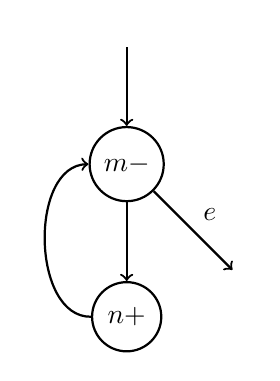
\begin{tikzpicture}[auto]
\tikzstyle{every path}=[thick];
\node (start) {};
\node[state] (subm) [below=of start] {$m{-}$};
\node (end) [below right=of subm] {};
\node[state] (addn) [below=of subm] {$n{+}$};
\path[->] (start) edge (subm);
\path[->] (subm) edge (addn);
\path[->] (subm) edge node {$e$} (end);
\path[->] (addn) edge [bend left=90] (subm);
\end{tikzpicture}
\end{center}

\ss{5.2}
\ms Suppose $x$ is stored in register $n$.  The following abacus
machine will put $\mathrm{sg}(x)$ in register $m$, assumed empty to begin with.

\begin{center}
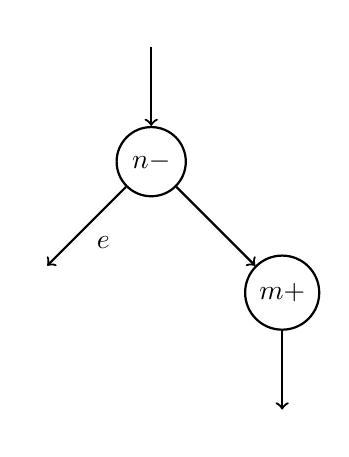
\begin{tikzpicture}[auto]
\tikzstyle{every path}=[thick];
\node (start) {};
\node[state] (subn) [below=of start] {$n{-}$};
\node[state] (addm) [below right=of subn] {$m{+}$};
\node (end1) [below=of addm] {};
\node (end2) [below left=of subn] {};
\path[->] (start) edge (subn);
\path[->] (subn) edge (addm);
\path[->] (addm) edge (end1);
\path[->] (subn) edge node {$e$} (end2);
\end{tikzpicture}
\end{center}
\ss{5.3}
\ms Since we know that exponentiation and subtraction are abacus computable, we know that $f(x)=1-0^x$ is abacus computable.  But this is equal to
$\mathrm{sg}(x)$, since $1-0^0 = 0$ but $1-0^x = 1$ for $x>0$.

Adam's solution: $x\dotdiv (x\dotdiv 1)$.
\ss{5.4} Adam: Hint out of mere laziness, it's the same as finding out whether the difference of two numbers is positive.  
\ss{5.5 and 5.6}
\ms I think this is right, but haven't 100\% thought it through. $x$ and $y$ are as in the problem, $y'$, $r$, and $q$ are initially 0.  After the machine halts, the remainder should be in $r$ (solving 5.5) and the quotient should be in $q$ (solving 5.6).

\begin{center}
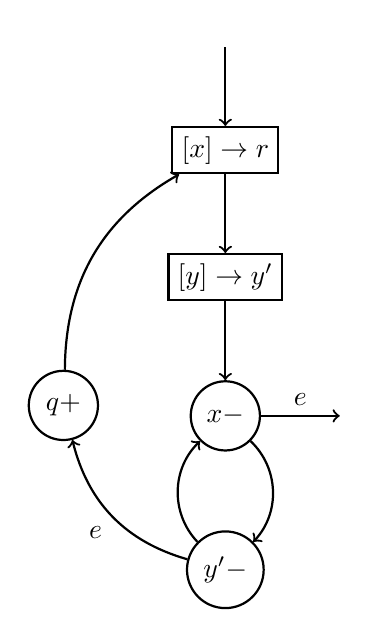
\begin{tikzpicture}[auto]
\tikzstyle{every path}=[thick];
\node (start) {};
\node[rectangle,draw] (xtor) [below=of start] {$[x]\to r$};
\node[rectangle,draw] (ytoyp) [below=of xtor] {$[y]\to y'$};
\node[state] (addq) [below left=of ytoyp] {$q{+}$};
\node[state] (subx) [below=of ytoyp] {$x{-}$};
\node (end1) [right=of subx] {};
\node[state] (subyp) [below=of subx] {$y'{-}$};
\path[->] (start) edge (xtor);
\path[->] (xtor) edge (ytoyp);
\path[->] (ytoyp) edge (subx);
\path[->] (subx) edge node {$e$} (end1);
\path[->] (subx) edge [bend left=45] (subyp);
\path[->] (subyp) edge [bend left=45] (subx);
\path[->] (subyp) edge [bend left=30] node {$e$} (addq);
\path[->] (addq) edge [bend left=30] (xtor);
\end{tikzpicture}
\end{center}

\ss{5.7} Adam: It’s a machine that first deletes what it’s scanning then finds the next
blank, makes it a stroke, makes the next stroke a blank and scans to the
end, and so on. In short it ``fills the gap" between all $k$ blocks and makes
a blank just to the right.
\ss{5.8} Adam: 1
\ss{5.9} Adam: First move everything right one position, as specified two questions above,
then run the program.
\ss{5.10} 
\pf First, create the equivalent Turing machine using the methods in section 5.2, then number them using the method on p. 36.

Adam: You could translate them into Turing machines which we know are coded
by natural numbers, or you could assign them to tuples coding the order
of their operations, the cells they’re operating on, and the instructions for
what to do next and what to do when empty. Then enumerate all such
machines as an enumeration of tuples.
\ss{5.11}
\ms This is a standard argument: let $d$ be the function as described in the problem, and let $\ulcorner d\urcorner$ be the natural number in the given encoding.  Then either $d(\ulcorner d\urcorner) = 0$ or $d(\ulcorner d\urcorner) = 1$.  Both cases are impossible by the definition of $d$.

\s{6 Recursive Functions}
% Some helper commands for the functionals defined in the text
\newcommand\id{\mathrm{id}} % identity
\newcommand\Cn{\mathrm{Cn}} % composition
\renewcommand\Pr{\mathrm{Pr}} % primitive recursion
\newcommand\Mn{\mathrm{Mn}} % minimization

% Get the dot over the minus for the modified difference function, this code was snagged from https://tex.stackexchange.com/questions/114188/special-character-dot-over-dash
\def\dotminus{\mathbin{\ooalign{\hss\raise1ex\hbox{.}\hss\cr
  \mathsurround=0pt$-$}}}

\ss{6.1}
Suppose $f(x,y)$ is recursive.
\sss{6.1(a)}
\ms Then $g(x,y) = f(y,x)$ is recursive by $g(x,y) = \Cn[f,\id^2_2,\id^2_1]$
\sss{6.1(b)}
\ms And $h(x) = f(x,x)$ is recursive by $h(x) = \Cn[f,\id^1_1,\id^1_1]$
\sss{6.1(c)} Adam: $k_{17}(x) = \Cn[f, const_{17}, id_1^2]$
\ss{6.2}
\ms $J(a,b)$ was defined as a polynomial in $a$ and $b$ divided by two.  Since we know that polynomials are primitive recursive (since multiplication and addition are), we'll be done if we can show that division by two is primitive recursive.

First we'll show that $\mathrm{isOdd}$ is primitive recursive, where $\mathrm{isOdd}(x)$ is 0 if $x$ is even and 1 if $x$ is odd.  Then $\mathrm{isOdd}$ can be defined by primitive recursion by $\mathrm{isOdd}(0) = 0$ and $\mathrm{isOdd}(x') = 1\dotminus\mathrm{isOdd}(x)$.

Then, division by two can be defined by $f(0) = 0$ and $f(x') = f(x) + \mathrm{isOdd}(x)$.
\ss{6.3}
\sss{6.3(a)} Adam: $x\dotdiv y + y\dotdiv x$
\sss{6.3(b)}
\ms From the fact that $x_{\leq}(x,y) = \mathrm{sg}(y\dotminus (x+1))$.
\sss{6.3(c)}
\mt I can definitely see a way of doing this if we assume that the pair coding and decoding functions are primitive recursive, but proving that the decoding functions are primitive recursive is not until 6.5, so I'm not sure if we're can use that here, or if the solution to that problem will depend on this one.

Adam: $\chi_{\leq}(x,y)\cdot y + \chi_{\leq}(y,x)\cdot x$
\ss{6.4}
\sss{6.4(a)}
\ms Using 6.3(a), $c(x,y,z) = 1\dotminus |x-yz|$
\sss{6.4(b)}
\ms Basically the same as part a.
\ss{6.5} Adam: We know from proposition 6.5 that sums up to $n$ are recursive.  Thus
    $\displaystyle K(n) = \sum_{i=1}^n \sum_{j=1}^n i\cdot d(n,i,j)$ and likewise
    for $L(n)$.  Essentially this just searches the $n\times n$ grid of the first
    few items in the array and, if any of them produces $n$ using the function
    $J$ then it reports the left coordinate.
\ss{6.6} Adam: To recall some of the ideas here,
    \begin{align*}
      1&=2^1(2\cdot 1-1)-1\\
      2&=2^0(2\cdot 2-1)-1\\
      3&=2^2(2\cdot 1-1)-1\\
      4&=2^0(2\cdot 3-1)-1\\
      5&=2^1(2\cdot 2-1)-1\\
      6&=2^0(2\cdot 4-1)-1\\
      7&=2^3(2\cdot 1-1)-1\\
      8&=2^0(2\cdot 5-1)-1\\
      9&=2^1(2\cdot 3-1)-1
    \end{align*}

    In general the pattern is to take any number, bump it up one, and get
    the biggest power of 2 that fits in it.  So for 6, if we bump it up 1 we get
    7, then the biggest power of 2 that fits in it is 0, and then pick $l(n)$
    based on that, which is 4.  If the number is 7 we bump it up to 8, find the
    biggest power of 2 that fits which is 3, and no other factor is left over
    so we pick $l(n)$ to be 1 in that case.  Hence $7=2^3(2\cdot 1-1)-1$.

    Of course with this picture in mind, every odd number has no powers of 2,
    so when we try to represent even numbers this way they will not use any
    powers of 2.  Hence $k(n)=0$ if $n$ is even.  Also for these even numbers
    we will just keep choosing bigger and bigger values of $l(n)$ to obtain the
    growth of the number.  That said it becomes obvious that in this case $l(n)$
    grows linearly and from the pattern in the few examples so far we can
    convince ourselves that $l(2m)=2m-1$.

    At that point you might notice other similar patterns like that every fourth
    power of 2 is 1.  Not every fourth power of 2 is 2, but that could have
    been predicted since it would fill up all the other spaces in the enumeration.
    If you draw it out you should find that every eigth power of 2 is 2 starting
    at the first instance, and every 16th power of 2 is 3, and so on.  In short
    $k(n)$ goes 1,0,2,0,1,0,3,0,1,0,2,0,1,0,4,0,... which is almost the same as
    another function we've seen just shifted around a bit.

    Returning to $l(n)$ it will also be linear for fixed $k(n)=c$.  We already
    saw this when $k(n)=c=0$ and it would also be true for $k(n)=1$ and so on.

    I won't attempt a more rigorous argument than this and will be happy if, at
    the meetup, anyone can make the answer more explicit.
\ss{6.7} Adam: Every function can be identified with a list of inputs and outputs
    of fixed size.  The set of all lists of length 1, 2, 3, and so on are each
    enumerable and the union of all lists of all lengths is an enumerable union
    of enumerable sets---using the basic technique by which we enumerate such a
    thing, we get an enumeration of recursive functions.
\ss{6.8}
\ms Standard self-reference/diagonalization argument
\ss{6.9}
\ms If it was, then $d$ from 6.8 would be recursive as $d(x) = h(x,x)$.

\s{7 Recursive Sets and Relations}
\ss{7.1}
\sss{7.1(a)}
\ms $S$ is given by $S(x,y)=\Cn[R,\id^2_2,\id^2_1]$, showing that if $R$ is primitive recursive (resp. recursive), then $S$ is primitive recursive (resp. recursive).  To show the result if $R$ is semirecursive, just carry an extra $t$ argument through.
\ss{7.2}
\ms We know that the relation $y^z\leq x$ is primitive recursive, since we know that exponentiation is primitive recursive from the 
last chapter.  $\mathrm{lg}(x, y)$ is the maximum $z$ for which
this is true.  In general, maximization isn't a primitive recursive or even a recursive operation, however we can put a bound on $z$: it can be no bigger than $x$, for example.  Thus we can use bounded maximization, which by Corollary 7.6, gives a primitive recursive function.
\ss{7.3}
\ms Use bounded minimization/maximization
\ss{7.5}
\ms First observe that the function $f(n)$ returning the minimum element of $A$ greater than or equal to $n$ is recursive by minimization.  Then $a(n)$ can be defined by $a(0) = f(0)$ and $a(n + 1) = f(a(n) + 1)$.
\ss{7.12}
\ss{7.13}
\ss{7.14}
\ss{7.15}
\ss{7.16}
\ss{7.17}

\s{8 Equivalent Definitions of Computability}
\ss{8.1}
\ms $\mathrm{strt}(x_1,x_2) = (2^{x_1+1}\dotminus 1)\cdot 2^{x_2+2}+(2^{x_2+1}\dotminus 1)$
\ss{8.2}
\end{document}
